\documentclass[conference]{IEEEtran}
\IEEEoverridecommandlockouts
% The preceding line is only needed to identify funding in the first footnote. If that is unneeded, please comment it out.
\usepackage{cite}
\usepackage{amsmath,amssymb,amsfonts}
\usepackage{algorithmic}
\usepackage{graphicx}
\usepackage{textcomp}
\usepackage{xcolor}
\usepackage{float}
\usepackage{url}
\def\BibTeX{{\rm B\kern-.05em{\sc i\kern-.025em b}\kern-.08em
		T\kern-.1667em\lower.7ex\hbox{E}\kern-.125emX}}
\begin{document}
	
	\title{Detection of Player Contact Events in NFL Games Using Analysis Systems
		\\
	}
	
	\author{\IEEEauthorblockN{Nahin José Peñaranda Mejia}
		\IEEEauthorblockA{\textit{Cod. 20231020032} \\
			\textit{Francisco José De Caldas University}\\
			Bogotá, Colombia\\
			njpenarandam@udistrital.edu.co}
		\and
		\IEEEauthorblockN{Nicolas Felipe Pulido Suarez}
		\IEEEauthorblockA{\textit{Cod. 20231020045} \\
			\textit{Francisco José De Caldas University}\\
			Bogotá, Colombia\\
			nfpulidos@udistrital.edu.co}
		\and
		\IEEEauthorblockN{Anderson David Arenas Gutierrez}
		\IEEEauthorblockA{\textit{Cod. 20231020030} \\
			\textit{Francisco José De Caldas University}\\
			Bogotá, Colombia\\
			adarenasg@udistrital.edu.co}
	}
	
	\maketitle
	
	\begin{abstract}
		In recent years, the accurate detection of physical contacts in sports environments has gained relevance, especially for improving player safety and performance analytics. This paper addresses the problem of detecting player-to-player and player-to-ground contacts in NFL games using a combination of video and sensor data. We propose a scalable, CPU-efficient system based on modular architecture, integrating computer vision and machine learning techniques. Our approach balances accuracy and performance under constrained hardware settings and chaotic real-game conditions. Results show that our lightweight solution can identify contact1s with promising precision and robustness, demonstrating the value of systems engineering in complex sports data scenarios.
	\end{abstract}
	
	\begin{IEEEkeywords}
		NFL, contact, kaggle, analysis, systems
	\end{IEEEkeywords}
	
	\section{Introduction}
	
	American football is a high-impact sport characterized by constant physical contact between players. These collisions, while integral to the game, pose significant risks including concussions, musculoskeletal injuries, and long-term health conditions. Because of this, player safety has become a growing concern, prompting efforts to monitor and analyze contact events more effectively. Traditional methods such as manual video review are time-consuming and error-prone, leading to a demand for automated systems that can detect and evaluate contact with higher accuracy and speed.
	
	The NFL Player Contact Detection competition hosted on Kaggle (https://www.kaggle.com/competitions/nfl-player-contact-detection) offers a data-rich platform to address this challenge. It provides video footage from multiple camera angles, high-frequency tracking data collected via sensors, and human-labeled contact annotations. The main task is to predict whether a physical contact occurred between players (or with the ground) at a given moment during a game. This involves aligning multimodal data streams, managing data imbalance due to the rarity of contact events, and coping with variations in video quality, sensor noise, and environmental factors.
	
	Several solutions submitted to the competition used powerful deep learning architectures for object detection and temporal modeling, often relying on GPU-based training and inference. While these approaches yielded high accuracy, they also presented barriers in terms of computational cost and reproducibility on lower-resource systems.
	
	Moreover, the challenge is not just technical but also systemic: contact events are influenced by dynamic player interactions, game context, and environmental noise, making the problem highly complex. A robust system must be capable of processing large volumes of data in near-real time while maintaining accuracy and interpretability, even when inputs vary significantly in quality or format. Synchronizing different data types—such as sensor streams and video frames—is a nontrivial task, and small misalignments can lead to major errors in prediction.
	
	From an engineering perspective, tackling this problem requires more than just selecting effective models. It involves designing an end-to-end pipeline that is modular, efficient, and adaptable to new datasets or deployment environments. This includes planning for scalability, managing resource limitations, and incorporating feedback mechanisms that help the system evolve over time.
	
	In this context, our approach focuses not only on implementing components of a detection pipeline, but also on understanding the structure and behavior of the system as a whole. Using principles from systems engineering, we carried out an analysis to identify the system’s key elements, interactions, and vulnerabilities. This analysis was performed in two stages, structured as academic workshops, where we combined technical experimentation with structured design thinking.
	
	This paper documents our initial efforts to replicate and simplify part of the top-performing solutions using CPU-friendly tools and a systems engineering perspective. The focus is on understanding the structure and dynamics of the proposed system through systems thinking and modeling techniques, as applied in two university workshops. Our catch-up phase emphasizes system design, sensitivity analysis, and prototype implementation under real-world constraints. The following sections describe the design approach and early validation proce
	
	\section{Methods and Material}
	
	The system design follows a modular pipeline architecture to ensure maintainability and scalability. Key components include data ingestion, preprocessing, player detection and tracking, feature extraction, contact prediction, and monitoring.
	
	\begin{figure*}[!t]
		\centering
		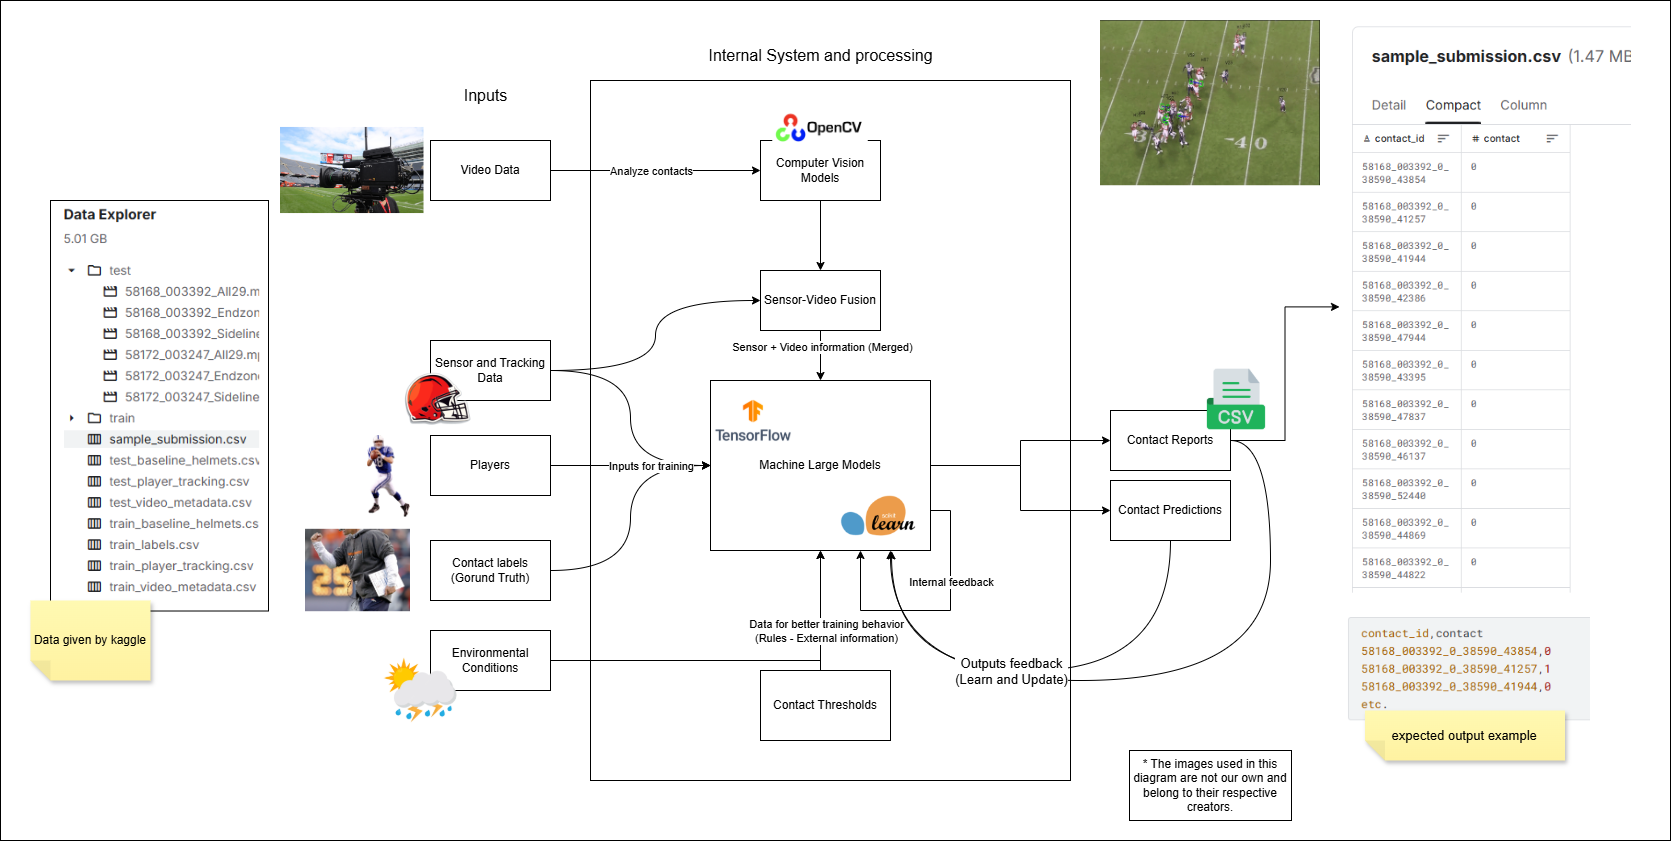
\includegraphics[width=1\textwidth]{Workshop2_diagram.png} % Ajusta el ancho según necesites
		\caption{Diagram of full system}
		\label{fig:imagen_centrada}
	\end{figure*}
	
	\subsection{Analysis Design}
	
	
	The systems analysis identified several key challenges that need to be addressed in the design. First, the data quality varies, with sensor inaccuracies and low video frame rates making it harder to extract reliable information. The system also should process data in real time, which is demanding on computational resources. Synchronizing sensor and video data is another challenge, as both must be perfectly aligned in time to ensure accuracy. Additionally, rare events, like significant player contacts, create imbalanced data that is difficult for models to handle. 
	
	The dataset is rich and includes sensor data, video feeds, and contact labels, but this complexity brings problems. Tracking players in crowded scenes or during fast movements is difficult, and environmental factors, like lighting or obstructions, can reduce video quality. Ground truth labels are essential for training the system, but errors or inconsistencies in these labels can cause issues later in the process. 
	
	The system also faces challenges related to combining different types of data. Sensor and video data need to be merged carefully to avoid errors, and the system’s accuracy depends on fine-tuned thresholds for decision-making. Random factors, like players overlapping or external conditions, make the system less predictable. 
	
	To address chaotic interactions and noise, we apply data augmentation and temporal smoothing. Regularization techniques like dropout, as well as ensemble modeling strategies, are considered to improve model generalization. Monitoring includes basic logging and performance tracking using the Observer design pattern.
	
	To solve these problems, the design should include tools for efficient real-time data processing, techniques for combining sensor and video data, and models that can handle imbalanced data and unexpected situations. This will make the system more reliable, scalable, and easy to maintain. 
	
	\begin{table*}[!t]
		\caption{Technical Stack and Justification for CPU-friendly Implementation}
		\centering
		\begin{tabular}{|p{3cm}|p{4cm}|p{6cm}|}
			\hline
			\textbf{Category} & \textbf{Tool/Library} & \textbf{Justification} \\
			\hline
			Programming Language & Python & Extensive data science ecosystem, widely accessible. \\
			\hline
			Data Processing & Pandas, NumPy & Efficient for sensor data manipulation, low memory footprint. \\
			\hline
			Video Processing & OpenCV & Lightweight for frame extraction and tracking, CPU-optimized. \\
			\hline
			Machine Learning & TensorFlow (MobileNet SSD) & Pre-trained, lightweight object detection model suitable for CPU. \\
			\hline
			Machine Learning & Scikit-learn (RandomForest) & Efficient for contact classification, minimal resource requirements. \\
			\hline
			Execution & Jupyter Notebooks & Interactive, user-friendly for workshops, supports step-by-step execution. \\
			\hline
			Version Control & Git & Standard for code versioning, lightweight and essential. \\
			\hline
			
		\end{tabular}
		\label{tab:tech_stack}
	\end{table*}
	
	\subsection{Technical Stack}
	
	Data ingestion handles video and sensor sources. Preprocessing synchronizes these streams using timestamp alignment, a critical step due to differing sampling frequencies (video at 30fps, sensors at 100Hz). For detection, we use MobileNet SSD, a lightweight object detection model suitable for CPU inference. Tracking is performed using OpenCV's CSRT algorithm, allowing us to maintain consistent player identities across frames.
	
	Feature extraction involves spatial and temporal metrics, such as proximity, velocity, and direction changes, derived from both video and sensor inputs. Contact prediction is handled by a RandomForestClassifier from Scikit-learn, chosen for its interpretability and solid performance with imbalanced data.
	
	All code is expected to develop in Jupyter notebooks and VS code for ease of testing and explanation during workshops. Git was used for version control. The system be to test locally on CPU hardware to ensure feasibility under limited computational resources.
	
	\newpage
	\section*{Results}
	
	This section is under construction...
	
	\section*{Conclusion}
	
	This paper presents the preliminary design and implementation phase of a system to detect player contacts in NFL games, based on the Kaggle competition data. While final testing and metrics are pending, the current work establishes a solid foundation.
	
	Our design emphasizes modularity, resource efficiency, and adaptability to real-game complexity. The use of systems thinking to guide architecture and decision-making has been key to identifying critical points and future challenges. Next steps include scaling up testing, optimizing performance, and exploring deployment scenarios for real-time or batch analysis in sports analytics.
	
	\begin{thebibliography}{00}
		\bibitem{b1} Kaggle, “NFL Player Contact Detection,” [Online]. Available: \url{https://www.kaggle.com/competitions/nfl-player-contact-detection}.
		\bibitem{b2} N. Nghia, “1st Place Solution - Kaggle NFL Player Contact Detection,” GitHub repository, [Online]. Available: \url{https://github.com/nvnnghia/1st_place_kaggle_player_contact_detection}.
		\bibitem{b3} OpenCV Developers, “OpenCV: Open Source Computer Vision Library,” [Online]. Available: \url{https://opencv.org}.
		\bibitem{b4} Scikit-learn Developers, “Random Forest Classifier,” [Online]. Available: \url{https://scikit-learn.org/stable/modules/generated/sklearn.ensemble.RandomForestClassifier.html}.
		\bibitem{b5} TensorFlow Developers, “MobileNet SSD - TensorFlow Object Detection API,” [Online]. Available: \url{https://github.com/tensorflow/models}.
		\bibitem{b6} Python Software Foundation, “Python Language Reference,” [Online]. Available: \url{https://www.python.org}.
		\bibitem{b7} Project Jupyter, “Jupyter Notebook Documentation,” [Online]. Available: \url{https://jupyter.org/documentation}.
		\bibitem{b8} Git SCM, “Git: Distributed Version Control System,” [Online]. Available: \url{https://git-scm.com}.
		\bibitem{b9} Repository for sources from workshops \url{https://github.com/ItzNxhin/SAD---Nahin-Nicolas-and-Anderson}
	\end{thebibliography}
	
	
\end{document}